% =====================================================================
% ARCHIVED SCM material — structural causal model interpretation of the
% confounding function c(x).
% Moved out of METHODOLOGY_SM.tex on 2026-06-19.
% Contains two sections: the reduced structural reading (label sm:scm)
% and the expanded SCM/DAG treatment (label sm:scm-full).
% Kept for reference only. Not \input by any compiled document, and not
% self-contained: it references assumptions, equations, and the
% confounding-function definition from the main text.
% =====================================================================

\section{Structural interpretation of the confounding function}\label{sm:scm}

\paragraph{Context and goal.}
The main text treats the RWD as potentially confounded without specifying the source of the confounding.
The confounding function $c(x)$ was defined in \eqref{eq:cf} as the residual bias in the RWD treated-versus-control contrast that the causal effect $\tau$ does not explain.
This is an operational definition: it says how to compute $c$ from the observed conditional means, but it says nothing about what real-world mechanisms generate the bias.

The aim of this section is to give $c(x)$ a causal-mechanistic interpretation.
We achieve this by introducing a latent random vector $U \in \mathcal{U}$, called the \emph{unmeasured confounder}, which stands in for any prognostic factor that affects survival but was not recorded in $X$.
Examples include frailty, comorbidities, biomarkers, performance status, genotype, and behavioural risk.
Under a structural model that lets $U$ enter the baseline and the treatment effect, the confounding function decomposes into two interpretable terms: an imbalance in the baseline prognostic function between the RWD treatment arms, and a term capturing effect modification by $U$.

The decomposition has three uses.
First, it makes precise what $c(x)$ measures in causal terms.
Second, it identifies the conditions under which $c(x)$ vanishes.
This in turn motivates the shrinkage prior placed on $c$ in the modelling section.
Third, it provides an entry point for sensitivity analyses that bound the magnitude of $c$ in terms of properties of $U$.

\paragraph{Structural outcome model.}
We posit an outcome equation on the log-time scale:
\begin{equation}
\log T(a) \;=\; f_0(X, U) \,+\, a\,\tau^*(X, U) \,+\, \varepsilon, \qquad \varepsilon \,\ind\, (X, U, A, S).
\label{eq:scm}
\end{equation}
The components have the following meanings.
$X \in \mathcal{X}$ is the vector of observed pre-treatment covariates introduced in the main text.
$U \in \mathcal{U}$ is the latent vector of unmeasured covariates described above; it is unknown to the analyst and never enters the likelihood used for inference.
$f_0(X, U)$ is the baseline log-transformed survival under control, that is, the conditional mean of $\log T(0)$ given $(X, U)$.
$\tau^*(X, U) = \E[\log T(1) - \log T(0) \mid X, U]$ is the treatment effect on the log scale conditional on the full covariate vector $(X, U)$.
$\varepsilon$ is an exogenous mean-zero error, independent of $(X, U, A, S)$; its distribution is left unspecified and follows the same flexible nonparametric form used in the main text.
The CATE on the log scale arises as the conditional mean of $\tau^*$ over $U$ given $X$:
\begin{equation}
\tau(x) \;=\; \E[\tau^*(X, U) \mid X = x].
\label{eq:cate-marginal}
\end{equation}
The model imposes additive separability of the baseline and the treatment effect.
It does not restrict the joint distribution of $(X, U, A)$ in the RWD, so the RWD remains free to be confounded through $U$.

\paragraph{Structural form of $c(x)$.}

\begin{proposition}[Structural form of the confounding function]\label{prop:cf-structural}
Under the structural model \eqref{eq:scm} and Assumptions~\ref{ass:sutva}--\ref{ass:transport}, the confounding function admits the decomposition:
\begin{equation}
c(x) \;=\; \underbrace{\E[f_0(X, U) \mid X = x, A = 1, S = 0] - \E[f_0(X, U) \mid X = x, A = 0, S = 0]}_{\text{prognostic imbalance}} \,+\, \underbrace{\delta_\tau(x)}_{\text{effect modification by }U},
\label{eq:cf-structural}
\end{equation}
where:
\begin{equation}
\delta_\tau(x) \;=\; \E[\tau^*(X, U) \mid X = x, A = 1, S = 0] \,-\, \tau(x).
\label{eq:delta-tau}
\end{equation}
\end{proposition}

\begin{proof}
Consistency (Assumption~\ref{ass:sutva}) gives $\log T = \log T(A)$ for every observation.
We evaluate the two conditional expectations entering the definition \eqref{eq:cf} of the confounding function.
In the RWD treated arm:
\begin{equation}
\E[\log T \mid X = x,\, A = 1,\, S = 0] \;=\; \E\bigl[f_0(X, U) + \tau^*(X, U) + \varepsilon \,\big|\, X = x,\, A = 1,\, S = 0\bigr],
\end{equation}
and in the RWD control arm:
\begin{equation}
\E[\log T \mid X = x,\, A = 0,\, S = 0] \;=\; \E\bigl[f_0(X, U) + \varepsilon \,\big|\, X = x,\, A = 0,\, S = 0\bigr].
\end{equation}
The error term contributes zero in both expressions because $\varepsilon$ has mean zero and is independent of $(X, U, A, S)$.
The difference of the two expectations is
\begin{multline}
\E[\log T \mid X = x,\, A = 1,\, S = 0] \,-\, \E[\log T \mid X = x,\, A = 0,\, S = 0] \\
\;=\; \E\bigl[f_0(X, U) \,\big|\, X = x,\, A = 1,\, S = 0\bigr] \,-\, \E\bigl[f_0(X, U) \,\big|\, X = x,\, A = 0,\, S = 0\bigr] \\
\,+\, \E\bigl[\tau^*(X, U) \,\big|\, X = x,\, A = 1,\, S = 0\bigr].
\end{multline}
We subtract $\tau(x)$ from both sides and apply the definition \eqref{eq:cf} of $c(x)$.
The result is \eqref{eq:cf-structural}, with $\delta_\tau(x)$ as in \eqref{eq:delta-tau}.
\end{proof}

\paragraph{Reduction under no unobserved effect modification.}
The structural form simplifies sharply when the treatment effect does not depend on $U$.

\begin{corollary}[Reduction to prognostic imbalance]\label{cor:no-effect-mod}
If $\tau^*(X, U)$ depends on the covariates only through $X$, i.e.\ $\tau^*(X, U) = \tau(X)$, then $\delta_\tau(x) = 0$ and the confounding function reduces to:
\begin{equation}
c(x) \;=\; \E[f_0(X, U) \mid X = x,\, A = 1,\, S = 0] \,-\, \E[f_0(X, U) \mid X = x,\, A = 0,\, S = 0].
\label{eq:cf-baseline}
\end{equation}
\end{corollary}

\begin{proof}
If $\tau^*(X, U) = \tau(X)$, then $\E[\tau^*(X, U) \mid X = x,\, A = 1,\, S = 0] = \tau(x)$, so $\delta_\tau(x) = 0$.
Substitution into \eqref{eq:cf-structural} yields \eqref{eq:cf-baseline}.
\end{proof}

\paragraph{Interpretation of the two components.}
The two pieces of \eqref{eq:cf-structural} have distinct substantive meanings.

The \emph{prognostic imbalance} term reflects that treated and control observations in the RWD differ in their distribution of $U$ given $X$.
Such an imbalance arises whenever treatment assignment in the RWD depends on unmeasured prognostic factors.
For example, suppose $U$ encodes frailty.
At the same observed covariate value $x$, frailer patients are less likely to be assigned the treatment.
Then $U$ is on average lower in the RWD treated arm than in the RWD control arm at the same $x$, and the conditional expectations of $f_0(X, U)$ differ across arms.
The sign and magnitude of the imbalance depend on the strength of the $U$-$A$ association and on the dependence of $f_0$ on $U$.

The term $\delta_\tau(x)$ captures \emph{effect modification by $U$}.
It is non-zero only when $\tau^*$ itself depends on $U$ and the distribution of $U$ given $X$ in the treated RWD arm differs from that in the population.
For intuition, suppose treatment works better for patients with a certain unmeasured trait.
If the RWD selectively treats patients with that trait, the RWD treated arm exhibits a stronger effect than the population CATE.
This piece is identically zero under Corollary~\ref{cor:no-effect-mod}.

\paragraph{When does the confounding function vanish?}
By Proposition~\ref{prop:cf-structural}, $c(x) = 0$ at $x$ whenever both the prognostic imbalance and $\delta_\tau(x)$ vanish.
A simple sufficient condition is the unmeasured-confounder independence $U \,\ind\, A \mid X, S = 0$: the unmeasured covariate is balanced across RWD treatment arms conditional on $X$.
This is the standard no-unmeasured-confounding assumption in the RWD.
Our framework deliberately avoids assuming it; the role of $c(x)$ is precisely to absorb the bias when this independence fails.

\paragraph{Implications for modelling and sensitivity.}
The structural form has two implications for what follows.
First, $c(x)$ is small when prognostic imbalance is mild and effect modification by $U$ is weak.
The shrinkage prior on $c$ \textbf{[PLACEHOLDER: to be introduced in the modelling section]} is then well-justified.
Second, the magnitude of $c(x)$ admits a sensitivity-analysis interpretation: bounds on how strongly $U$ is associated with $A$ in the RWD and with $f_0$ translate into bounds on $c(x)$.
\textbf{[PLACEHOLDER: brief discussion of relevant sensitivity-analysis frameworks (e.g., Rosenbaum, E-values, Robins--Rotnitzky) and where they fit in the paper.]}



\newpage
\section{Structural causal model interpretation of the confounding function (expanded)}\label{sm:scm-full}

\paragraph{Context and goal.}
The previous section interprets $c(x)$ through a structural outcome model.
That model is silent on how the other variables in the problem are generated.
It posits a functional form for $\log T(a)$ but leaves the mechanisms behind $X$, $U$, $S$, and $A$ unspecified.
The main-text assumptions, Assumptions~\ref{ass:sutva}--\ref{ass:transport}, carry the remaining structure as conditional independencies.

We give here a fuller treatment via a structural causal model \citep[SCM;][]{pearl2009causality, peters2017elements}.
An SCM specifies a structural equation for every endogenous variable and a joint distribution over exogenous noises.
The resulting framework is still very broad.
It is also a sub-class of the regression model used for inference in the main text.
The SCM has three advantages over the outcome-model treatment.
First, it makes the data-generating mechanism explicit.
Second, it lets us recover the main-text assumptions from a small set of structural conditions.
Third, it provides a mechanism-level language for sensitivity analyses on $c(x)$.

\paragraph{The structural causal model.}
We posit the following SCM over the random vector $(X, U, S, A, T)$:
\begin{equation}
\begin{aligned}
X &\;=\; f_X(N_X),\\
U &\;=\; f_U(X, N_U),\\
S &\;=\; f_S(X, N_S),\\
A &\;=\; f_A(X, U, S, N_A),\\
T &\;=\; f_T(X, U, A, N_T).
\end{aligned}
\label{eq:fscm}
\end{equation}
The exogenous noises $(N_X, N_U, N_S, N_A, N_T)$ are mutually independent.
The structural functions $f_X, \ldots, f_T$ are otherwise unrestricted.
We model the source $S$ as a function of $X$ alone, so that $N_U$ and $N_S$ are independent.
The latent vector $U$ enters every downstream equation, reflecting that we leave its causal role open.
The potential outcomes are obtained by intervention on $A$:
\begin{equation}
T(a) \;:=\; f_T(X, U, a, N_T), \qquad a \in \{0, 1\}.
\label{eq:fscm-po}
\end{equation}
The observational outcome equals $T(A)$ by construction, which recovers consistency.

We further restrict $f_T$ to admit an additive separation of the baseline and the treatment effect on the log-time scale:
\begin{equation}
\log T(a) \;=\; f_0(X, U) \,+\, a\,\tau^*(X, U) \,+\, \varepsilon,
\label{eq:fscm-outcome}
\end{equation}
where $\varepsilon = \varepsilon(N_T)$ has mean zero and is independent of $(X, U, A, S)$.
Equation~\eqref{eq:fscm-outcome} recovers the outcome model of the previous section.
The remaining equations in \eqref{eq:fscm} are new.
They expose the selection mechanism $f_S$ and the treatment-assignment mechanism $f_A$ that the outcome model left implicit.

\paragraph{Graphical representation.}
The SCM induces the directed acyclic graph in Figure~\ref{fig:scm-dag}.
The graph displays the causal mechanisms and makes the role of $U$ visible.
The arrow $U \to A$ is the source of confounding in the RWD.
The same arrow is degenerate in the RCT under the randomisation restriction below.

\begin{figure}[tb]
\centering
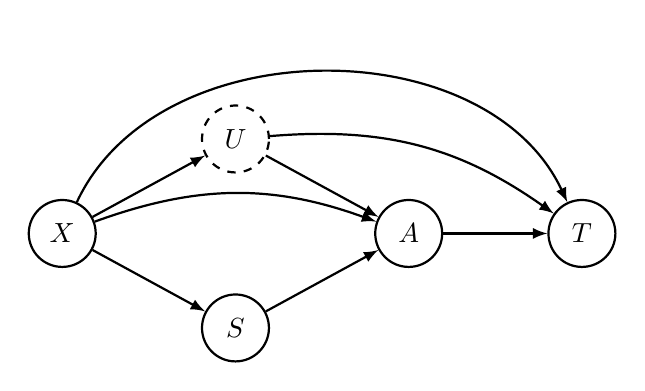
\begin{tikzpicture}[
  >=latex,
  obs/.style={circle, draw, thick, minimum size=0.85cm, inner sep=0pt},
  lat/.style={circle, draw, thick, dashed, minimum size=0.85cm, inner sep=0pt},
  arr/.style={->, thick}
]
  \node[obs] (X) at (0, 0)    {$X$};
  \node[lat] (U) at (2.2, 1.2) {$U$};
  \node[obs] (S) at (2.2, -1.2) {$S$};
  \node[obs] (A) at (4.4, 0)  {$A$};
  \node[obs] (T) at (6.6, 0)  {$T$};

  \draw[arr] (X) -- (U);
  \draw[arr] (X) -- (S);
  \draw[arr] (X) to[bend left=20] (A);
  \draw[arr] (X) to[bend left=65] (T);
  \draw[arr] (U) -- (A);
  \draw[arr] (U) to[bend left=20] (T);
  \draw[arr] (S) -- (A);
  \draw[arr] (A) -- (T);
\end{tikzpicture}
\caption{DAG implied by the SCM \eqref{eq:fscm}. Observed variables are solid; the unmeasured confounder $U$ is dashed. The arrow $U \to A$ is degenerate when $S = 1$ under the RCT randomisation restriction \eqref{eq:fscm-rct}.}
\label{fig:scm-dag}
\end{figure}

\paragraph{Recovering the main-text assumptions.}
Each of the main-text assumptions maps to an explicit constraint on the SCM.
We list them in turn.

\emph{Consistency (Assumption~\ref{ass:sutva})} holds by construction.
The structural equation for $T$ gives $T = f_T(X, U, A, N_T) = T(A)$.

\emph{Unconfoundedness of the RCT (Assumption~\ref{ass:rct-unconf})} restricts $f_A$ on the event $\{S = 1\}$.
The RCT mechanism does not depend on $U$:
\begin{equation}
f_A(X, U, 1, N_A) \;=\; f_A^{\mathrm{RCT}}(X, N_A).
\label{eq:fscm-rct}
\end{equation}
Together with the independence of $N_A$ from $(N_U, N_T)$, this restriction gives $A \,\ind\, (U, T(0), T(1)) \mid X, S = 1$.

\emph{Positivity (Assumption~\ref{ass:positivity-both})} requires that the conditional distribution of $A$ given $(X, S)$ have full support on $\{0, 1\}$ in both sources.
This is a non-degeneracy condition on $f_A$ jointly with the noise $N_A$.

\emph{Cross-source exchangeability (Assumption~\ref{ass:transport})} reduces to two conditions.
First, $f_T$ has no $S$ argument, so the conditional distribution of $T(a)$ given $(X, U)$ does not depend on $S$.
Second, the distribution of $U$ given $X$ is the same in both sources:
\begin{equation}
U \mid X, S = 1 \;\overset{d}{=}\; U \mid X, S = 0.
\label{eq:fscm-uxs}
\end{equation}
The second condition follows from our construction.
We let $S$ depend on $X$ but not on $N_U$, so $U \,\ind\, S \mid X$.
In the selection-diagram language of \citet{bareinboim2016causal}, $S$ acts as a selection node attached to $X$ but disconnected from $U$.

\emph{Conditionally independent censoring (Assumption~\ref{ass:censoring})} is a statement about the censoring mechanism.
It is separate from the outcome SCM and we treat it as outside \eqref{eq:fscm}.

\paragraph{The SCM as a sub-class of the regression model.}
The regression model \eqref{eq:aft-model} places nonparametric priors on the conditional-mean components $m_0$, $\tau$, and $c$.
It is agnostic about the joint distribution of $(X, U, A, S)$.
The SCM \eqref{eq:fscm}--\eqref{eq:fscm-outcome} is one particular family of data-generating processes compatible with that regression model.
Each component of the regression model arises as a conditional expectation under the SCM:
\begin{equation}
m_0(x, s) \;=\; \E[f_0(X, U) \mid X = x, S = s], \qquad \tau(x) \;=\; \E[\tau^*(X, U) \mid X = x],
\label{eq:fscm-induced}
\end{equation}
and $c(x)$ is the residual contrast defined by \eqref{eq:cf}.
The SCM family is still very broad.
It permits arbitrary nonlinear mechanisms, multivariate $U$ of unrestricted dimension, and arbitrary dependence of $A$ on $(X, U)$ in the RWD.
The only structural restrictions are the additive form \eqref{eq:fscm-outcome}, the source-symmetric outcome equation, and the independence \eqref{eq:fscm-uxs} of $U$ from $S$ given $X$.
The first restriction is the AFT modelling choice.
The latter two are precisely what cross-source exchangeability buys us.

\paragraph{Identification within the SCM.}
The identification result of Proposition~\ref{prop:ident} carries over without change.
The RCT slice of the SCM gives $\E[\log T \mid X, A = 1, S = 1] - \E[\log T \mid X, A = 0, S = 1] = \tau(X)$ via \eqref{eq:fscm-rct} and \eqref{eq:fscm-uxs}.
The RWD slice identifies $\tau(x) + c(x)$ as the observed treated-versus-control contrast.
The SCM contributes no additional identifying restrictions.
The latent vector $U$ remains unidentified.

\paragraph{Structural form of $c(x)$.}
We re-derive the structural form of the confounding function within the SCM.
The argument is the same as in Proposition~\ref{prop:cf-structural}.
The SCM makes the conditioning sets transparent.
Decompositions of this form go back to \citet{brumback2004sensitivity} for marginal structural models and \citet{vanderweele2011bias} for general outcomes.

\begin{proposition}[Structural form of $c$ under the SCM]\label{prop:cf-fscm}
Under the SCM \eqref{eq:fscm}--\eqref{eq:fscm-outcome} with restrictions \eqref{eq:fscm-rct} and \eqref{eq:fscm-uxs}, the confounding function satisfies
\begin{equation}
c(x) \;=\; \Delta f_0(x) \,+\, \delta_\tau(x),
\label{eq:cf-fscm}
\end{equation}
with the prognostic-imbalance term
\begin{equation}
\Delta f_0(x) \;=\; \E[f_0(X, U) \mid X = x, A = 1, S = 0] \,-\, \E[f_0(X, U) \mid X = x, A = 0, S = 0],
\label{eq:fscm-delta-f0}
\end{equation}
and the effect-modification term $\delta_\tau(x)$ defined as in \eqref{eq:delta-tau}.
\end{proposition}

\begin{proof}
We use \eqref{eq:fscm-outcome} and the mean-zero independence of $\varepsilon$ to write
\begin{align*}
\E[\log T \mid X{=}x, A{=}1, S{=}0]
  &\;=\; \E[f_0(X, U) + \tau^*(X, U) \mid X{=}x, A{=}1, S{=}0],\\
\E[\log T \mid X{=}x, A{=}0, S{=}0]
  &\;=\; \E[f_0(X, U) \mid X{=}x, A{=}0, S{=}0].
\end{align*}
Subtraction gives the RWD treated-versus-control contrast as a sum of two terms in $f_0$ and one term in $\tau^*$.
We subtract $\tau(x) = \E[\tau^*(X, U) \mid X = x]$ on both sides.
The definition \eqref{eq:cf} of $c(x)$ yields \eqref{eq:cf-fscm}.
\end{proof}

\paragraph{Structural conditions for $c \equiv 0$.}
The SCM lets us read off transparent sufficient conditions under which the confounding function vanishes.

\begin{corollary}[Structural conditions for vanishing $c$]\label{cor:c-zero-fscm}
Under the SCM, $c(x) \equiv 0$ if either of the following holds.
\begin{enumerate}[label=\textup{(\roman*)}]
\item The RWD treatment mechanism does not depend on $U$:
$f_A(X, U, 0, N_A) = f_A^{\mathrm{RWD}}(X, N_A)$.
\item Both $f_0$ and $\tau^*$ depend on covariates only through $X$.
\end{enumerate}
Either condition is sufficient. Neither is necessary.
\end{corollary}

\begin{proof}
Under (i), $U \,\ind\, A \mid X, S = 0$. The conditional distribution of $U$ given $(X, A, S = 0)$ does not depend on $A$. Both $\Delta f_0(x)$ and $\delta_\tau(x)$ vanish.
Under (ii), $f_0(X, U) = f_0(X)$ and $\tau^*(X, U) = \tau(X)$. The conditional expectations in \eqref{eq:cf-fscm} reduce to $f_0(x)$ and $\tau(x)$, so $\Delta f_0 \equiv 0$ and $\delta_\tau \equiv 0$.
\end{proof}

Condition (i) is the standard no-unmeasured-confounding assumption applied to the RWD.
Our framework does not impose it.
The confounding function exists precisely to absorb the bias when (i) fails.
Condition (ii) describes a setting in which $U$ is causally inert for the outcome.
In that case the latent $U$ can be marginalised away without loss.

\paragraph{Parametric instance.}
A linear-Gaussian instance of the SCM makes the structural sources of $c(x)$ tangible.
Take $f_0(X, U) = \beta_0 + \beta_X^\top X + \beta_U U$ and $\tau^*(X, U) = \gamma_0 + \gamma_X^\top X + \gamma_U U$.
Take an RWD treatment mechanism $\p(A = 1 \mid X, U, S = 0) = \Phi(\alpha_0 + \alpha_X^\top X + \alpha_U U)$, with $U \mid X \sim N(0, \sigma_U^2)$.
The two pieces of \eqref{eq:cf-fscm} become
\begin{equation}
\Delta f_0(x) \;=\; \beta_U\,\bigl\{\E[U \mid X{=}x, A{=}1, S{=}0] - \E[U \mid X{=}x, A{=}0, S{=}0]\bigr\},
\end{equation}
and
\begin{equation}
\delta_\tau(x) \;=\; \gamma_U\,\bigl\{\E[U \mid X{=}x, A{=}1, S{=}0] - \E[U \mid X{=}x]\bigr\}.
\end{equation}
Each conditional mean of $U$ in the RWD is a monotone function of $\alpha_U$.
The size of $c(x)$ is governed by three structural quantities.
The first is $\alpha_U$, the strength of confounding in the treatment mechanism.
The second is $\beta_U$, the baseline dependence on $U$.
The third is $\gamma_U$, the strength of effect modification by $U$.
Any one of them being zero kills the corresponding piece.
All three zero recovers $c(x) \equiv 0$.

\paragraph{Sensitivity-analysis framing.}
The SCM provides mechanism-level handles for sensitivity analysis.
Two structural quantities govern the magnitude of $c$.
The first is the dependence of $A$ on $U$ in the RWD, governed by $f_A(\cdot, \cdot, 0, \cdot)$.
The second is the dependence of $f_0$ and $\tau^*$ on $U$.
Standard sensitivity-analysis frameworks parameterise these quantities and induce bounds on the bias.
Rosenbaum bounds \citep{rosenbaum2002observational} constrain the odds-ratio dependence of $A$ on $U$.
The E-value of \citet{vanderweele2017evalue} summarises the joint association strength required to nullify an observed effect.
The framework of \citet{robins2000sensitivity} bounds the bias under prescribed deviations from ignorability.
\citet{YangLiuZengWang2025} apply confounding-function methods to a setting close to ours.
Each framework translates into an implied envelope on $c(x)$ via \eqref{eq:cf-fscm}.
The Bayesian counterpart of these analyses is the shrinkage prior on $c$ introduced in the modelling section.
The prior downweights large values of $c$ without ruling them out.
The data are free to pull $c$ away from zero where the bias is strong.

\paragraph{Implications for modelling.}
The SCM clarifies what the shrinkage prior on $c$ encodes.
Shrinkage towards zero is consistent with the structural picture in which $U$ is approximately balanced across RWD arms at most values of $X$ and effect modification by $U$ is mild.
The prior does not force these conditions.
The shrinkage strength controls how aggressively the RWD informs $\tau$ through the shared baseline $m_0$.
A weaker prior on $c$ trusts the RWD less.
A stronger prior on $c$ approximates the conventional no-unmeasured-confounding assumption in the RWD.
The full SCM treatment makes the prior interpretable as a soft version of Corollary~\ref{cor:c-zero-fscm}(i).
Related RCT--RWD fusion strategies that learn a confounding-bias function from a small experimental sample include \citet{Kallus2018} and \citet{YangLiuZengWang2025}.
